\documentclass[a4paper]{article}
\usepackage[utf8]{inputenc}
\usepackage[T1]{fontenc}
\usepackage[left=3cm, right=3cm]{geometry}
\usepackage{graphicx}
\usepackage{subcaption}
\usepackage{listings}
\usepackage{latexsym}
\usepackage{amsfonts}
\usepackage[hidelinks]{hyperref}
\usepackage{amssymb}
\usepackage{wasysym}
\usepackage[dvipsnames]{xcolor}

\newcommand{\command}[1]{\subsection{#1}}


\lstset{
  language=C++,
  basicstyle=\small\ttfamily,
  keywordstyle=\color{ForestGreen}\ttfamily,
  identifierstyle=\ttfamily,
  commentstyle=\color{gray}\ttfamily,
  stringstyle=\color{Purple}\ttfamily,
  showstringspaces=false,
  emph=[1]{std,vector,string,Eigen,Dense,VectorXd,bool,double,char,void},
  emphstyle=[1]{\color{blue}},
  moredelim=[is][\itshape]{[*}{*]}, % means: [* this will be highlighted in the code *] and this not. 
  moredelim=[is][\color{red}]{[**}{**]}
}


\begin{document}

\begin{center}
  \begin{huge}
    \textbf{The Figure Class\\}
  \end{huge}
  Basic plotting in C++
\end{center}
  
\vspace*{3cm}
  \tableofcontents
\vspace*{\fill}

\newgeometry{bottom=2cm, left=3cm, right=3cm}

\section{Opening example}

This short example code will show, how the Figure class can be used.
\begin{lstlisting}
# include <vector>
# include <Eigen/Dense>
# include <figure/figure.hpp>

int main()
{
  std::vector<double> x(10), y(10);
  for (int i = 0; i < 10; ++i){ 
    x[i] = i; y[i] = std::exp(-0.2*i)*std::cos(i));
  }
  Eigen::VectorXd u = Eigen::VectorXd::LinSpaced(500, 1, 10),
                  v = ( u.array().cos()*(-0.2*u).array().exp() ).matrix();
  [**mgl**]::[**Figure**] fig;
  fig.[**plot**](x, y, " +r").[**label**]("Sample Data");
  fig.[**plot**](u, v, "b").[**label**]("Function");
  fig.[**legend**]();
  fig.[**save**]("plot.eps");
  return 0;
}
\end{lstlisting}

\begin{figure}[h]
  \centering
  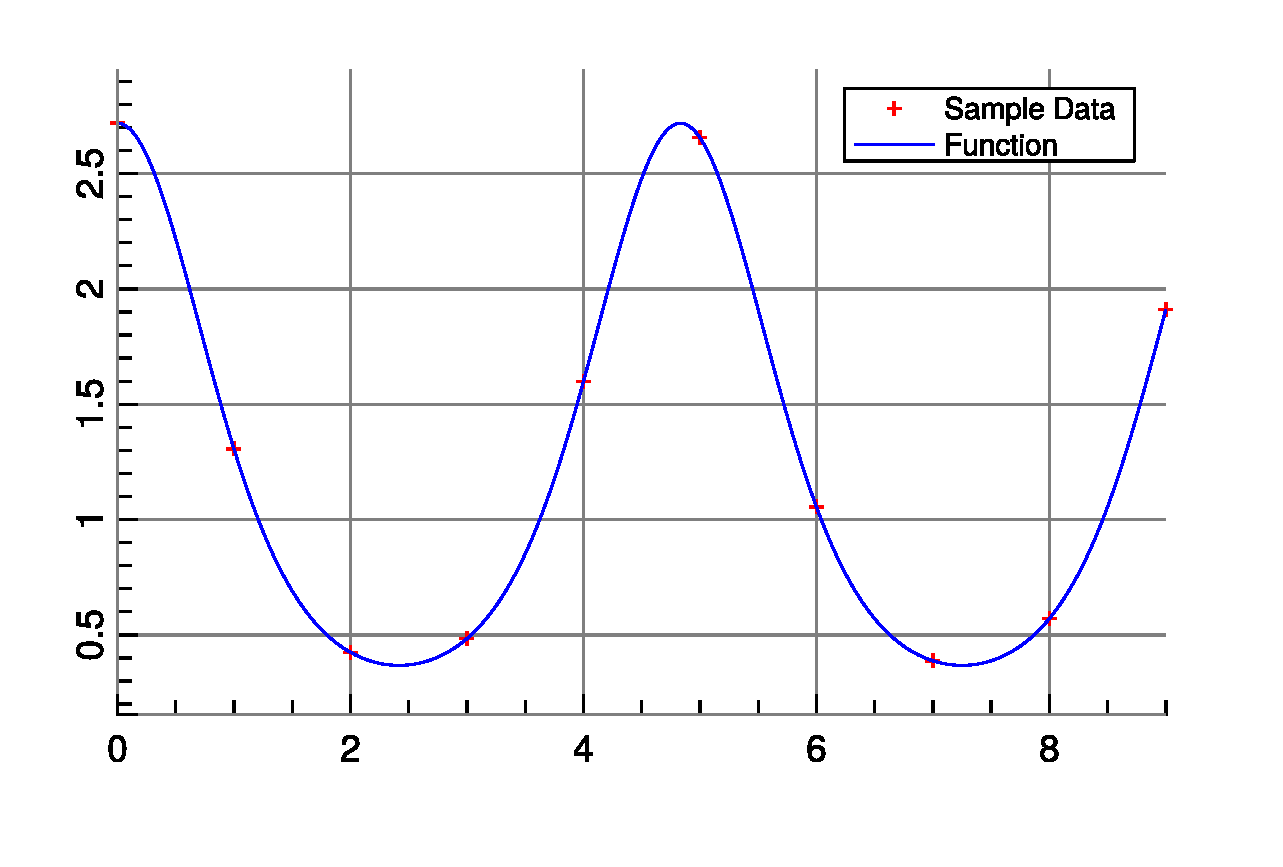
\includegraphics[width=0.6\textwidth]{./examples_from_doc/opening-example.eps}
  \thispagestyle{empty}
\end{figure}

\restoregeometry
\section{Methods}

\command{grid}

\textbf{Definition:}
\begin{lstlisting}
void grid( const bool& on = true, 
           const std::string& gridType = "-", 
           const std::string& gridCol = "h" )
\end{lstlisting}
%
\textbf{Restrictions:} None. \\ \\
%
\textbf{Examples:}
\begin{lstlisting}
  mgl::Figure fig;
  fig.plot(x, y);
  fig.[**grid**](false); // unset grid
  fig.save("plot.eps");

  mgl::Figure fig;
  fig.plot(x, y);
  fig.[**grid**](true, "!", "h"); // grey fine mesh
  fig.save("plot.eps");
\end{lstlisting}

\begin{figure}[h]
  \centering
  \begin{subfigure}[hb]{.32\linewidth}
    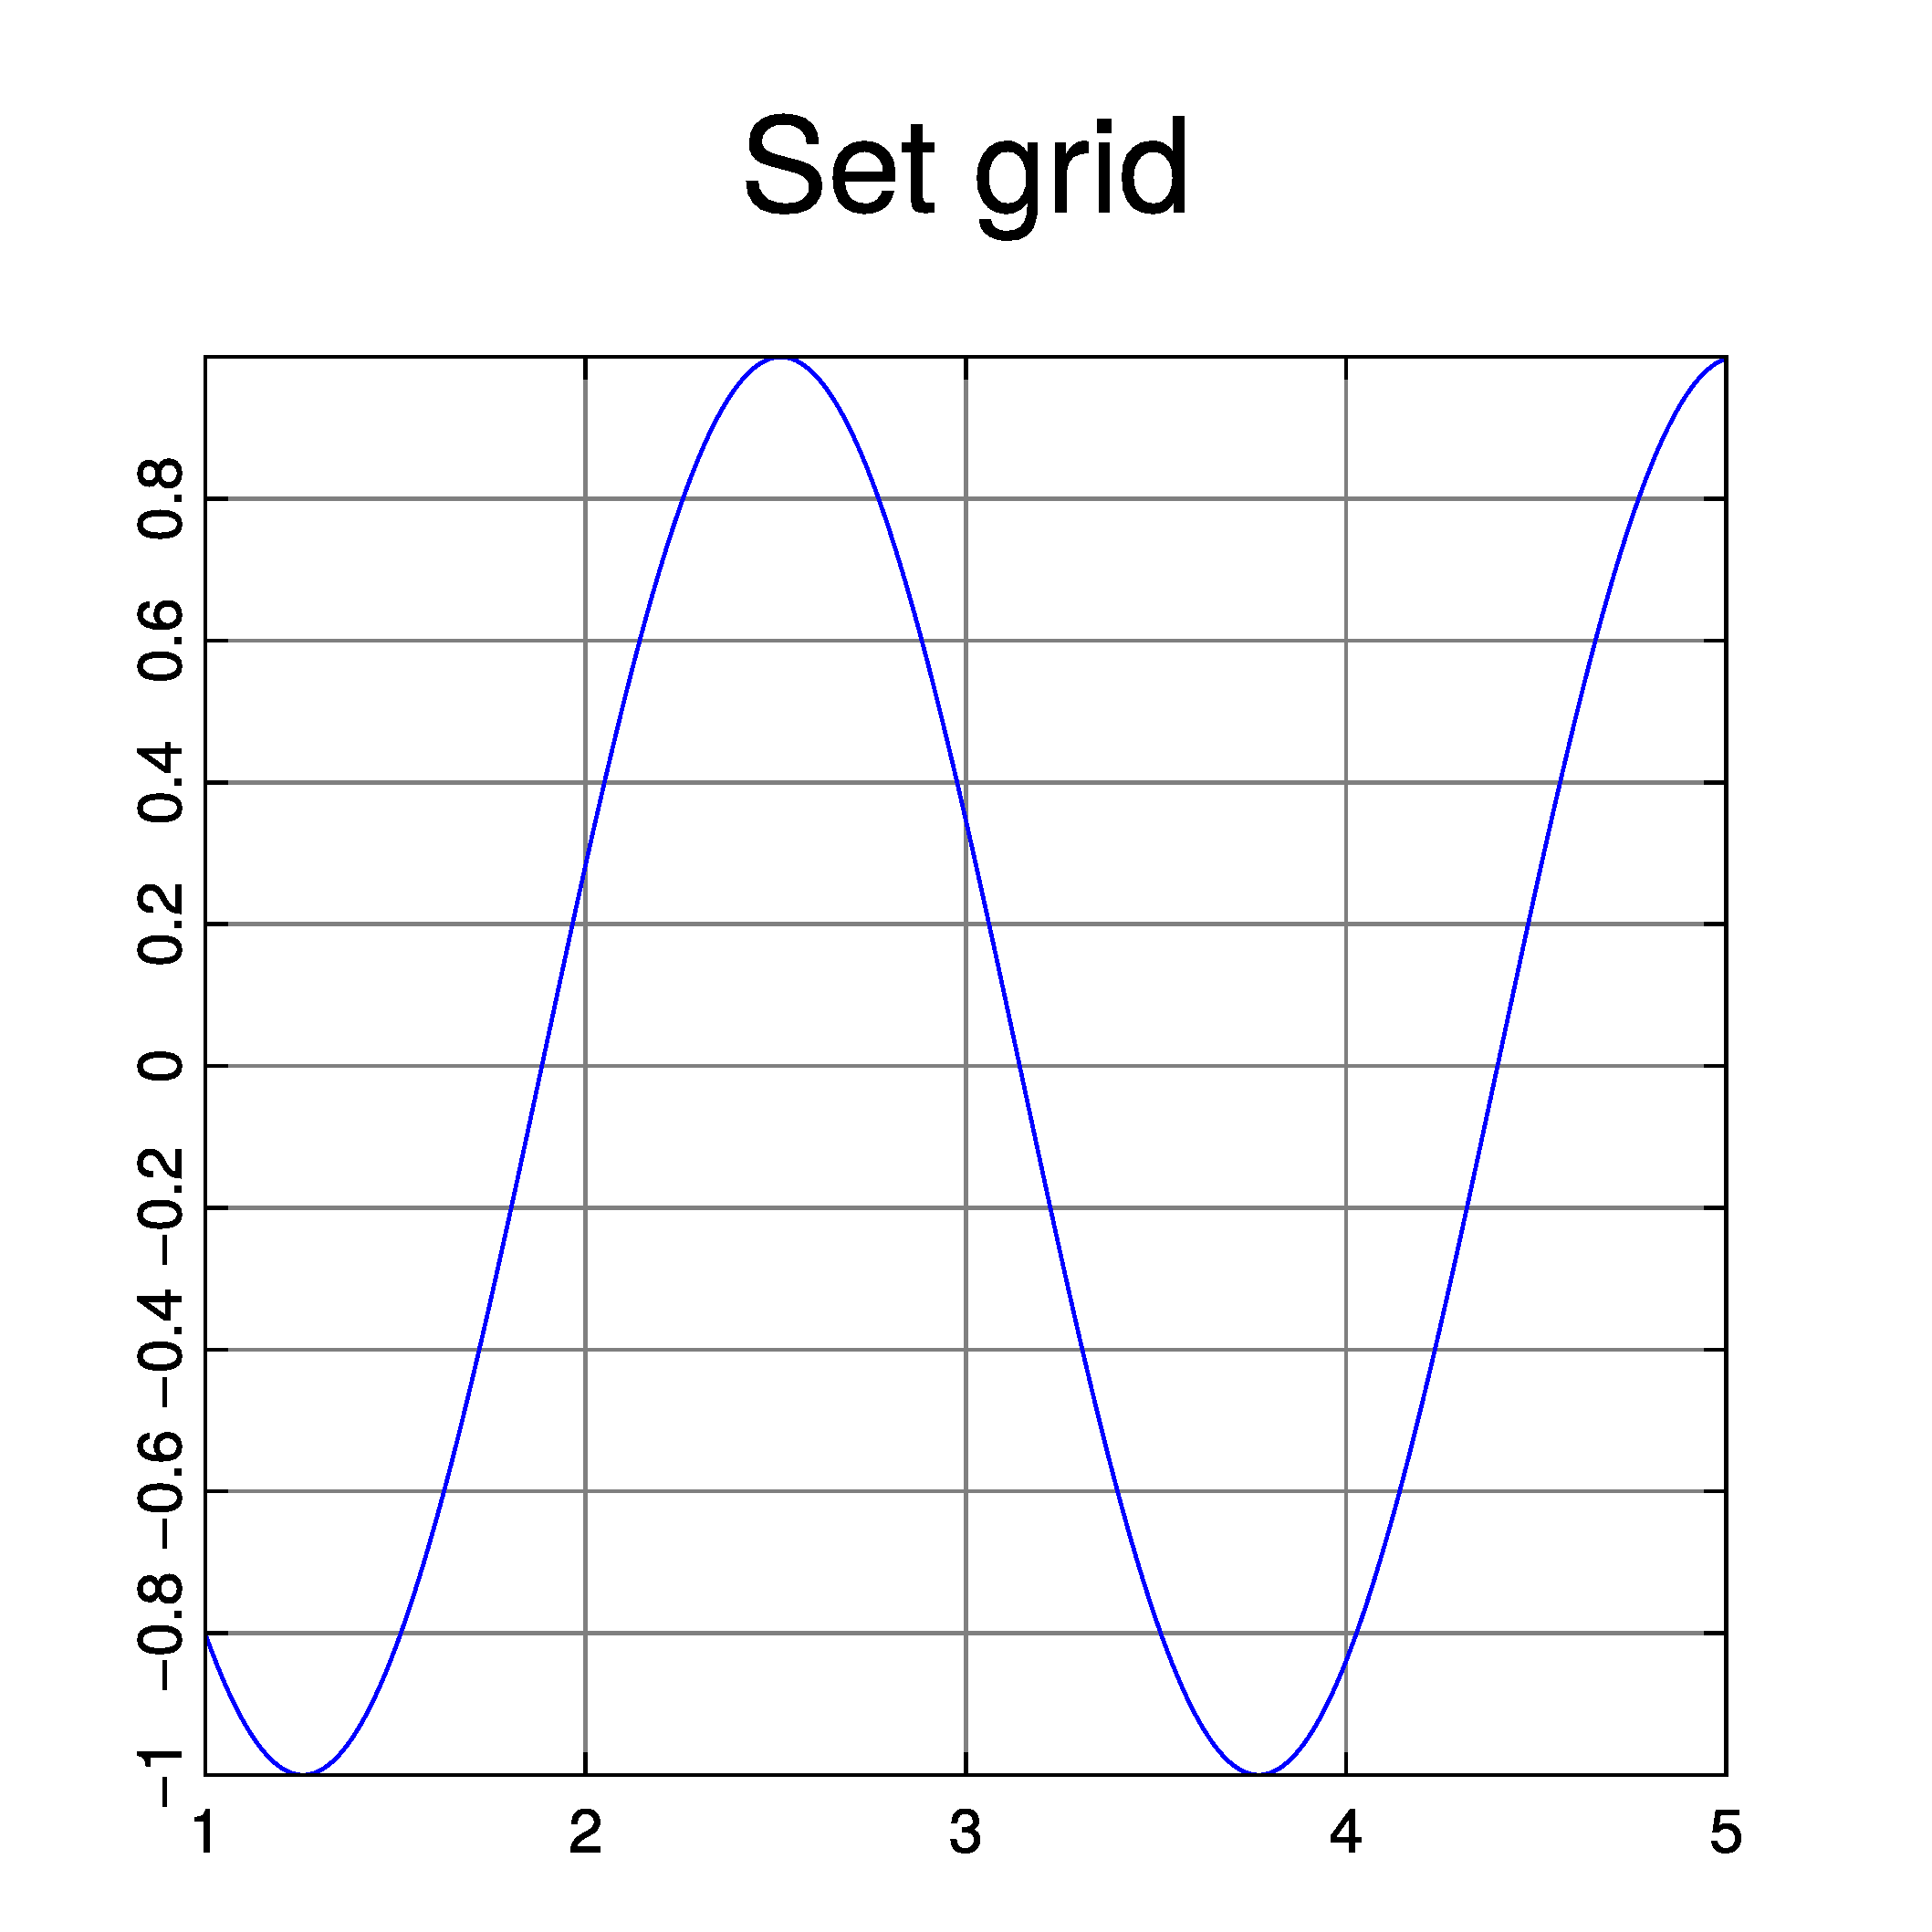
\includegraphics[width=\textwidth]{./examples_from_doc/grid/grid_1.eps}
  \end{subfigure}
    \hspace{2cm}
  \begin{subfigure}[hb]{.32\linewidth}
    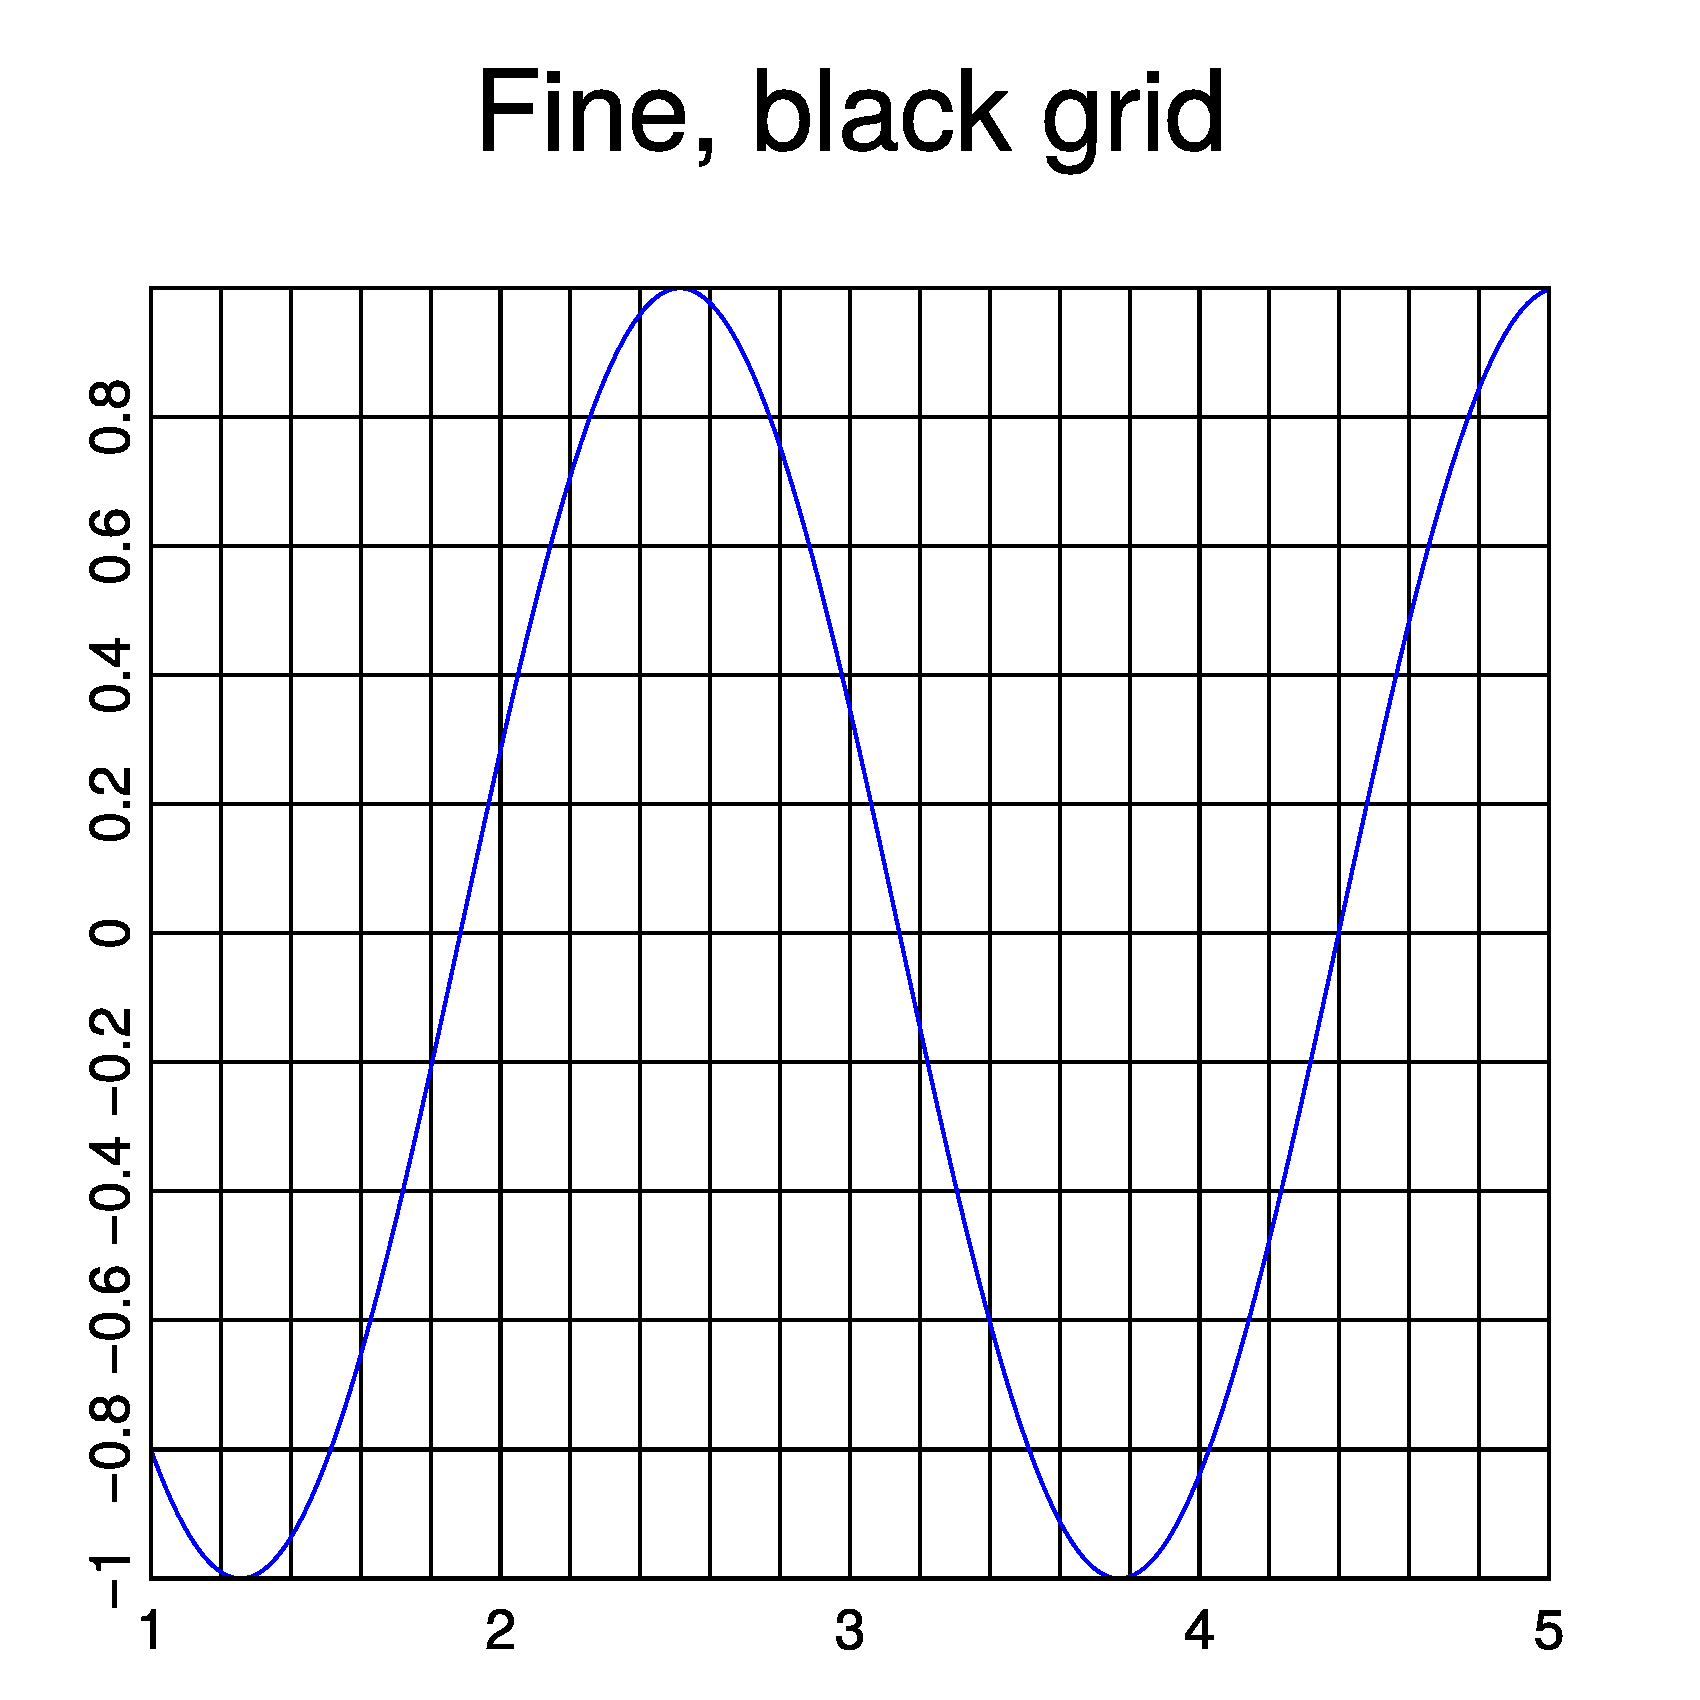
\includegraphics[width=\textwidth]{./examples_from_doc/grid/grid_2.eps}
  \end{subfigure}
\end{figure}

%%%%%%%%%
\newpage
%%%%%%%%%
\command{xlabel}

\textbf{Definition:}
\begin{lstlisting}
void xlabel( const std::string& label, 
             const double& pos = 0 )
\end{lstlisting}
%
\textbf{Restrictions:} None. \\ \\
%
\textbf{Examples:}
\begin{lstlisting}
  mgl::Figure fig;
  fig.plot(x, y, "g+"); // 'g+' equals matlab/python '+-g'
  fig.[**xlabel**]("Linear x axis");
  fig.save("plot.eps");

  mgl::Figure fig;
  fig.[**xlabel**]("Logarithmix x axis"); // no restricitons on call order
  fig.setlog(true, true);
  fig.plot(x, y, "g+");
  fig.save("plot.eps");
\end{lstlisting}

\begin{figure}[h]
  \centering
  \begin{subfigure}[hb]{.32\linewidth}
    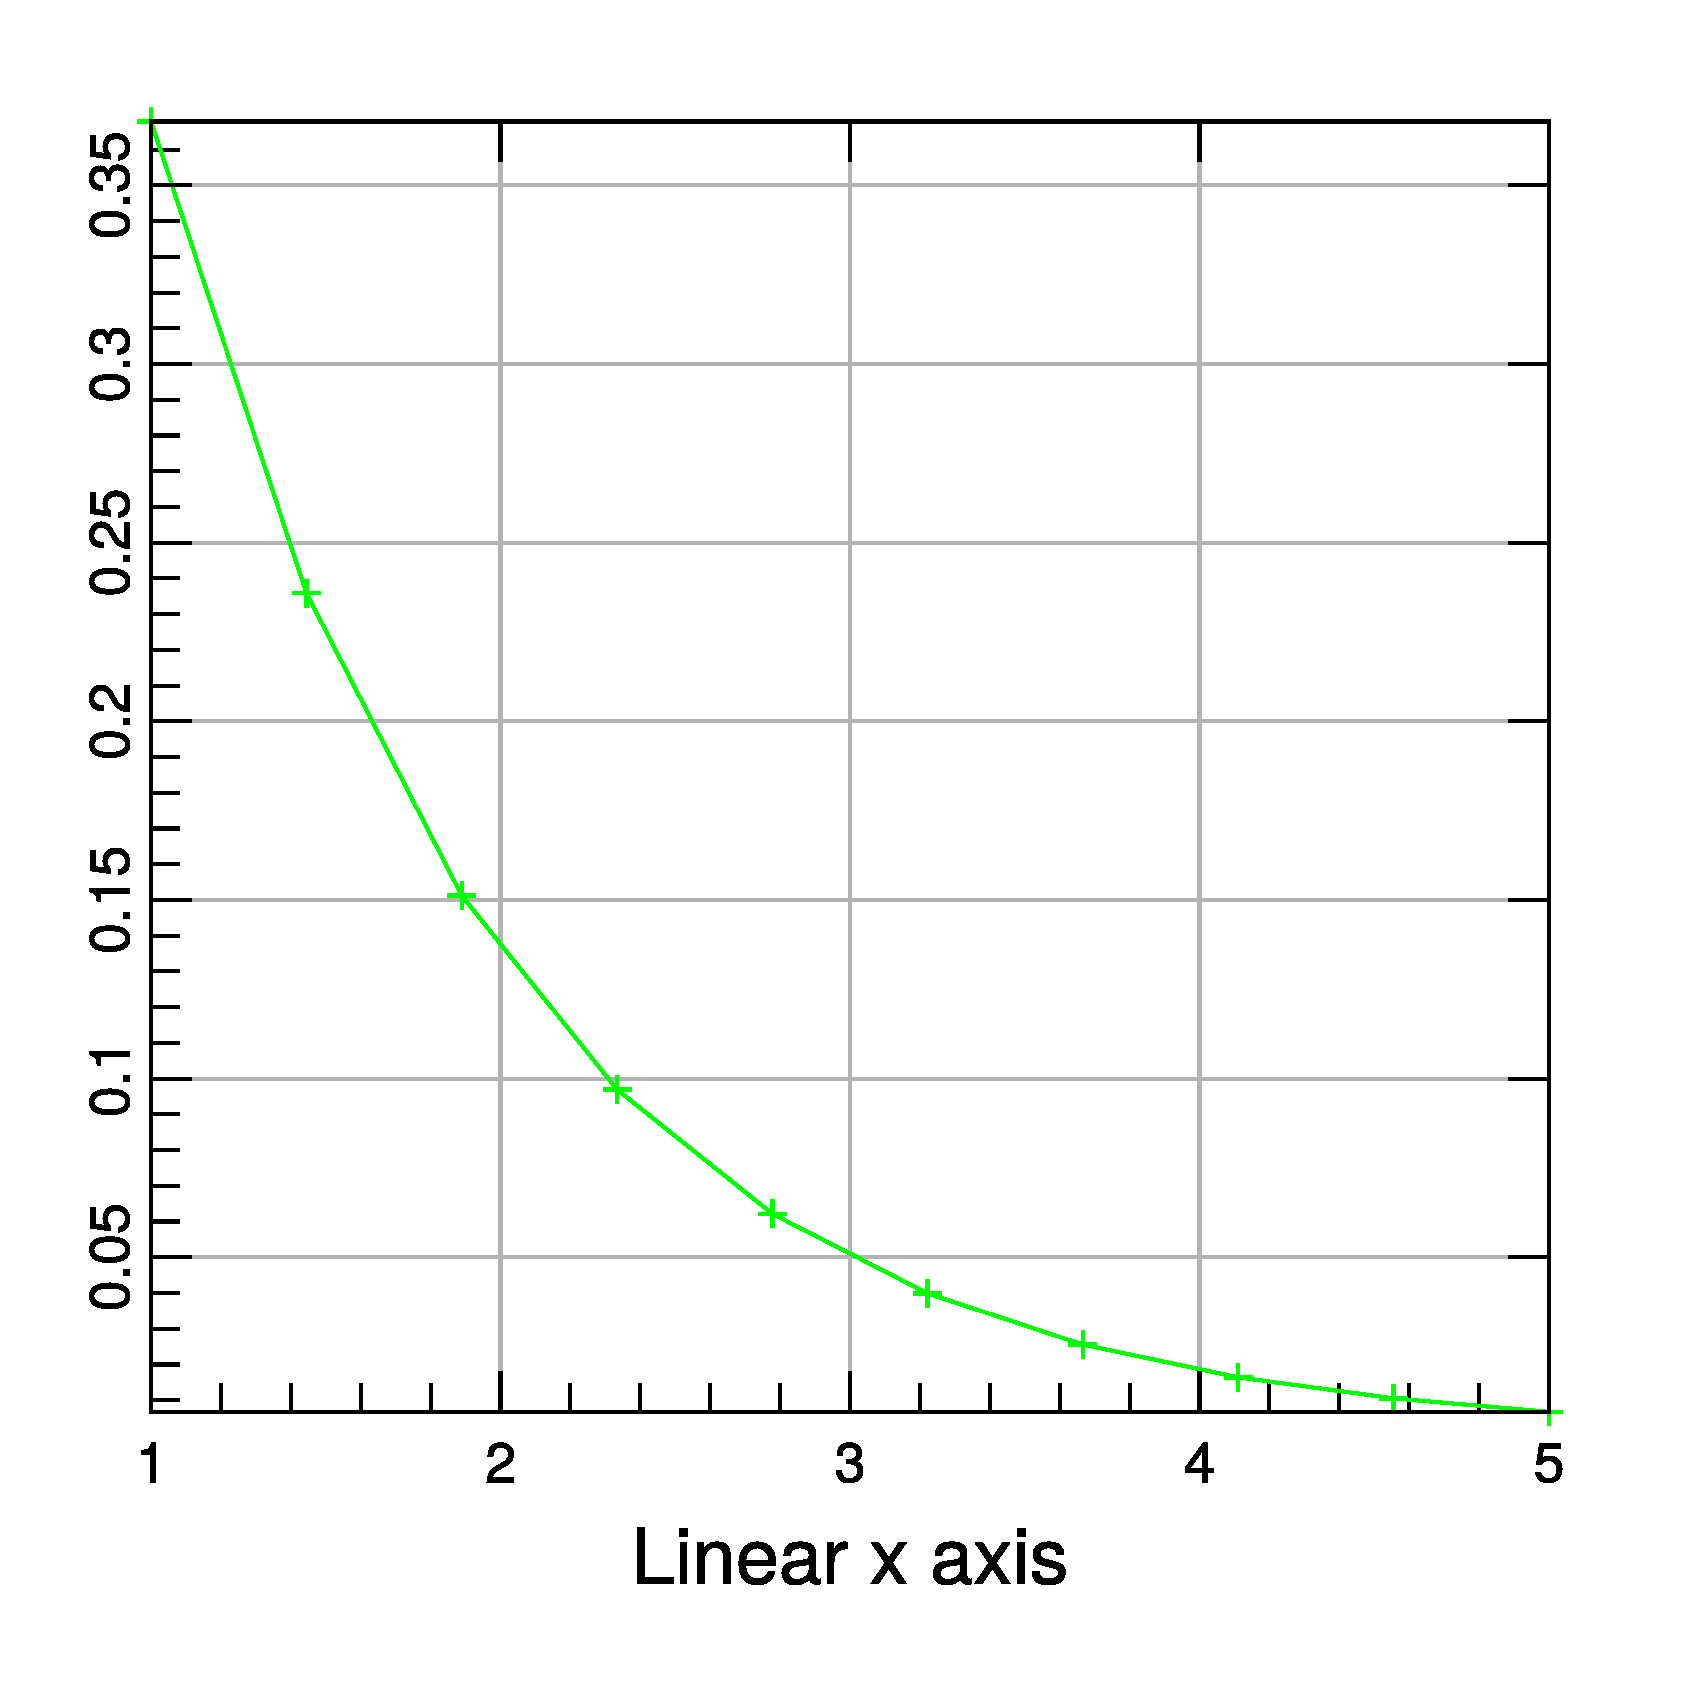
\includegraphics[width=\textwidth]{./examples_from_doc/xlabel/xlabel_1.eps}
  \end{subfigure}
  \hspace{2cm}
  \begin{subfigure}[hb]{.32\linewidth}
    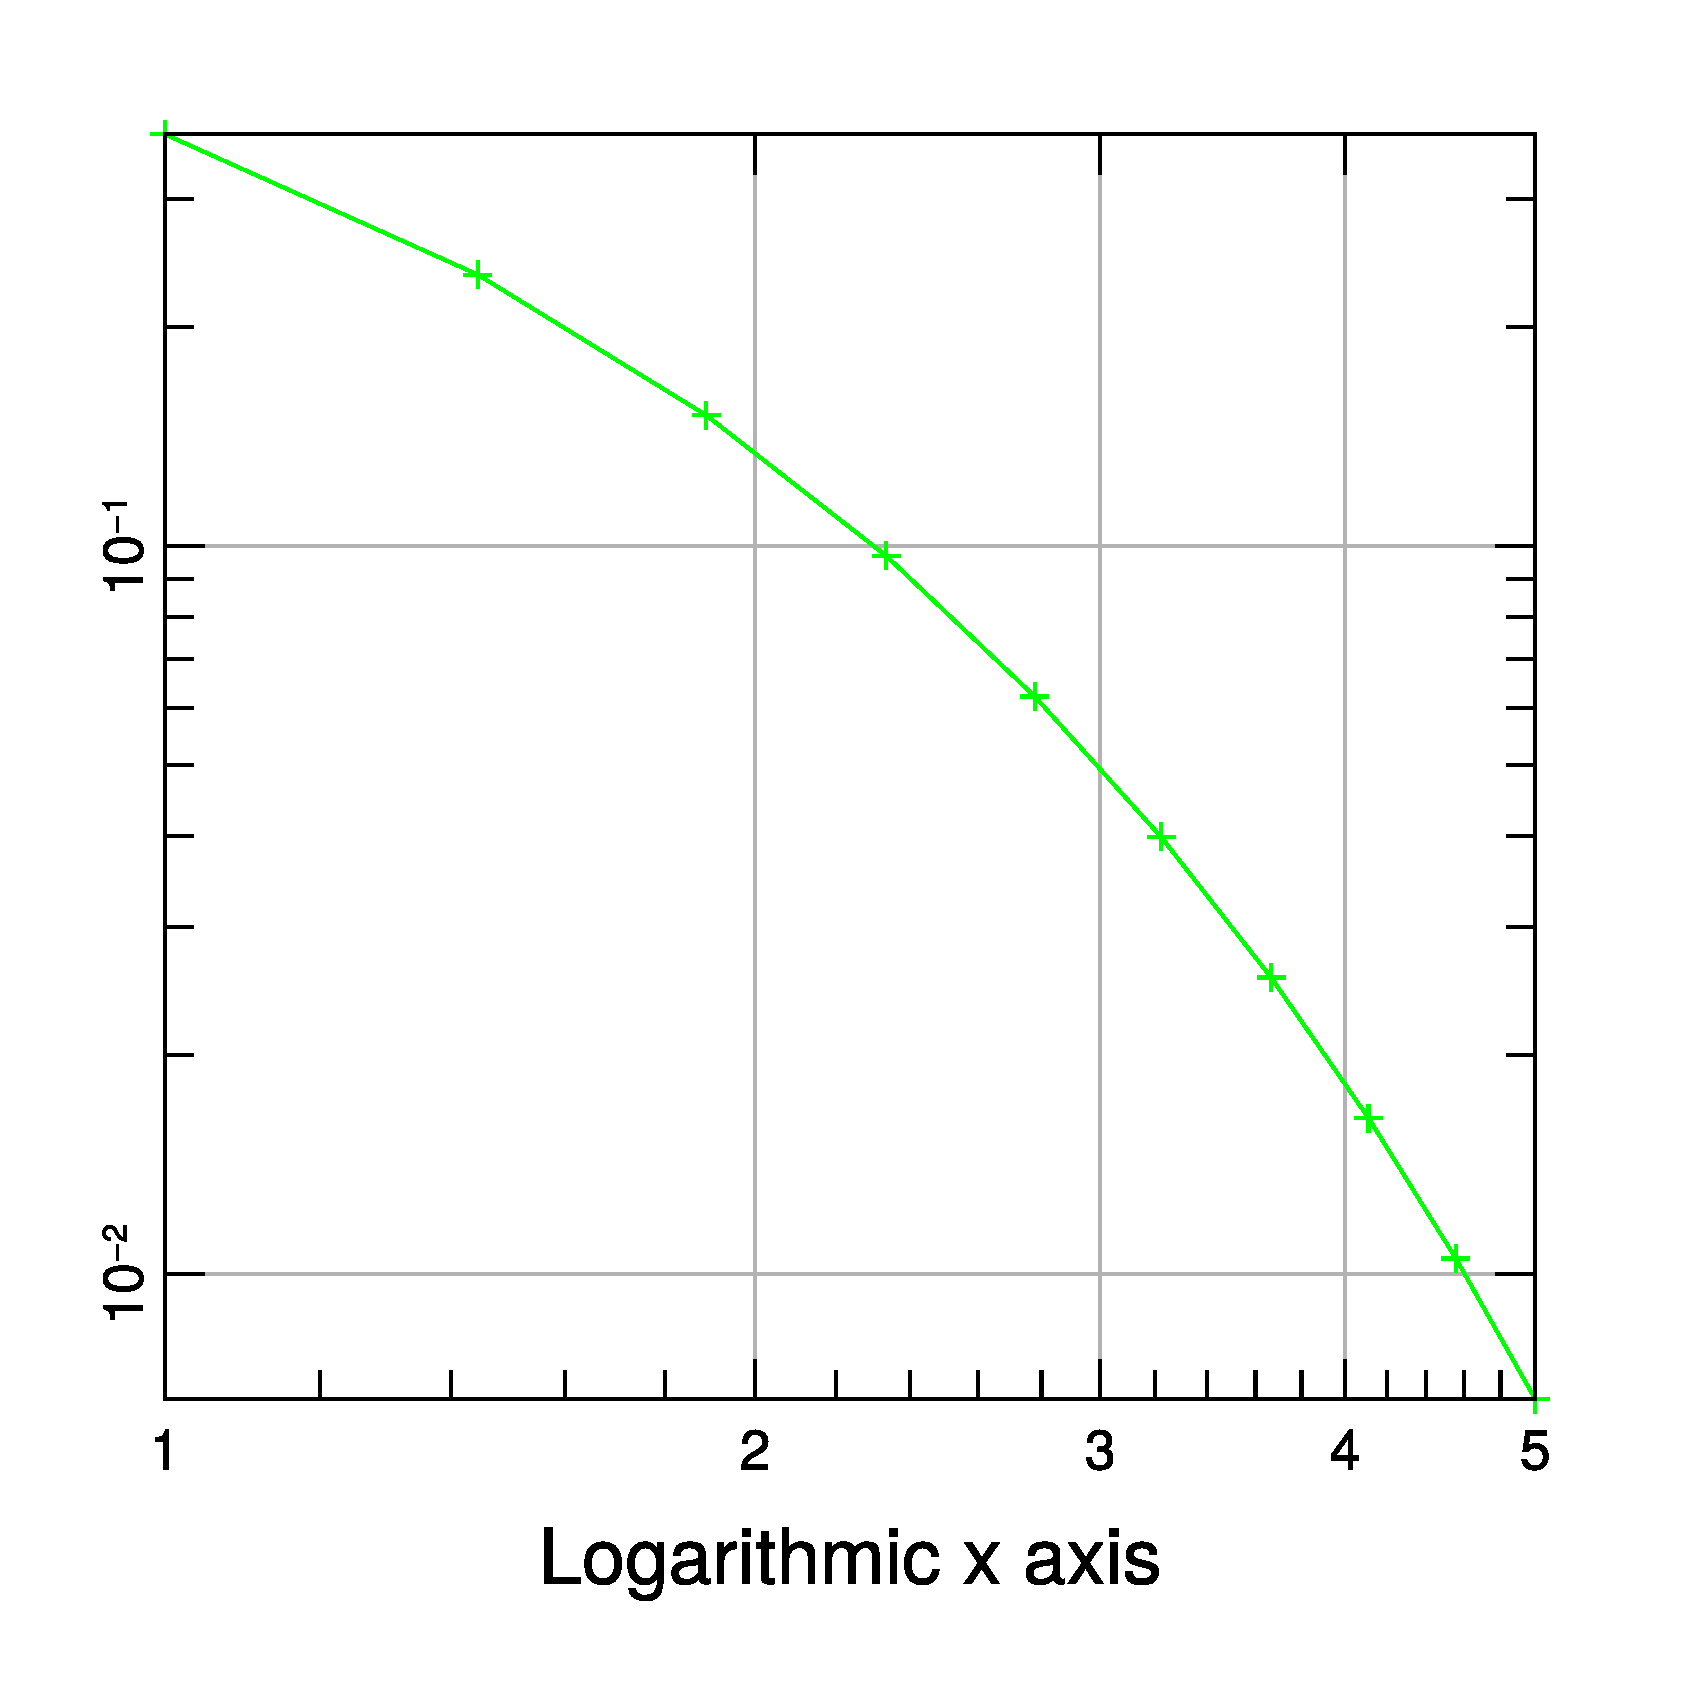
\includegraphics[width=\textwidth]{./examples_from_doc/xlabel/xlabel_2.eps}
  \end{subfigure}
\end{figure}

\command{ylabel}

\textbf{Definition:}
\begin{lstlisting}
void ylabel( const std::string& label, 
             const double& pos = 0 )
\end{lstlisting}
%
\textbf{Restrictions:} None. \\ \\
%
\textbf{Examples:} See \texttt{xlabel}.

%%%%%%%%%
\newpage
%%%%%%%%%
\command{legend}

\textbf{Definition:}
\begin{lstlisting}
void legend( const double& xPos = 1, 
             const double& yPos = 1 )
\end{lstlisting}
%
\textbf{Restrictions:} None.  \\ \\
%
\textbf{Examples:}
\begin{lstlisting}
  mgl::Figure fig;
  fig.plot(x0, y0).label("My Function");
  fig.[**legend**](); // 'activate' legend 
  fig.save("plot");
 
  mgl::Figure fig;
  fig.plot(x0, y0).label("My Function");
  fig.[**legend**](0.5, 0.25); // set position to (0.5, 0.25)
  fig.save("plot");

  mgl::Figure fig;
  fig.plot(x0, y0).label("My Function");
  fig.save("plot"); // legend won't appear as legend() hasn't been called
\end{lstlisting}

\begin{figure}[h]
  \centering
  \begin{subfigure}[hb]{.32\linewidth}
    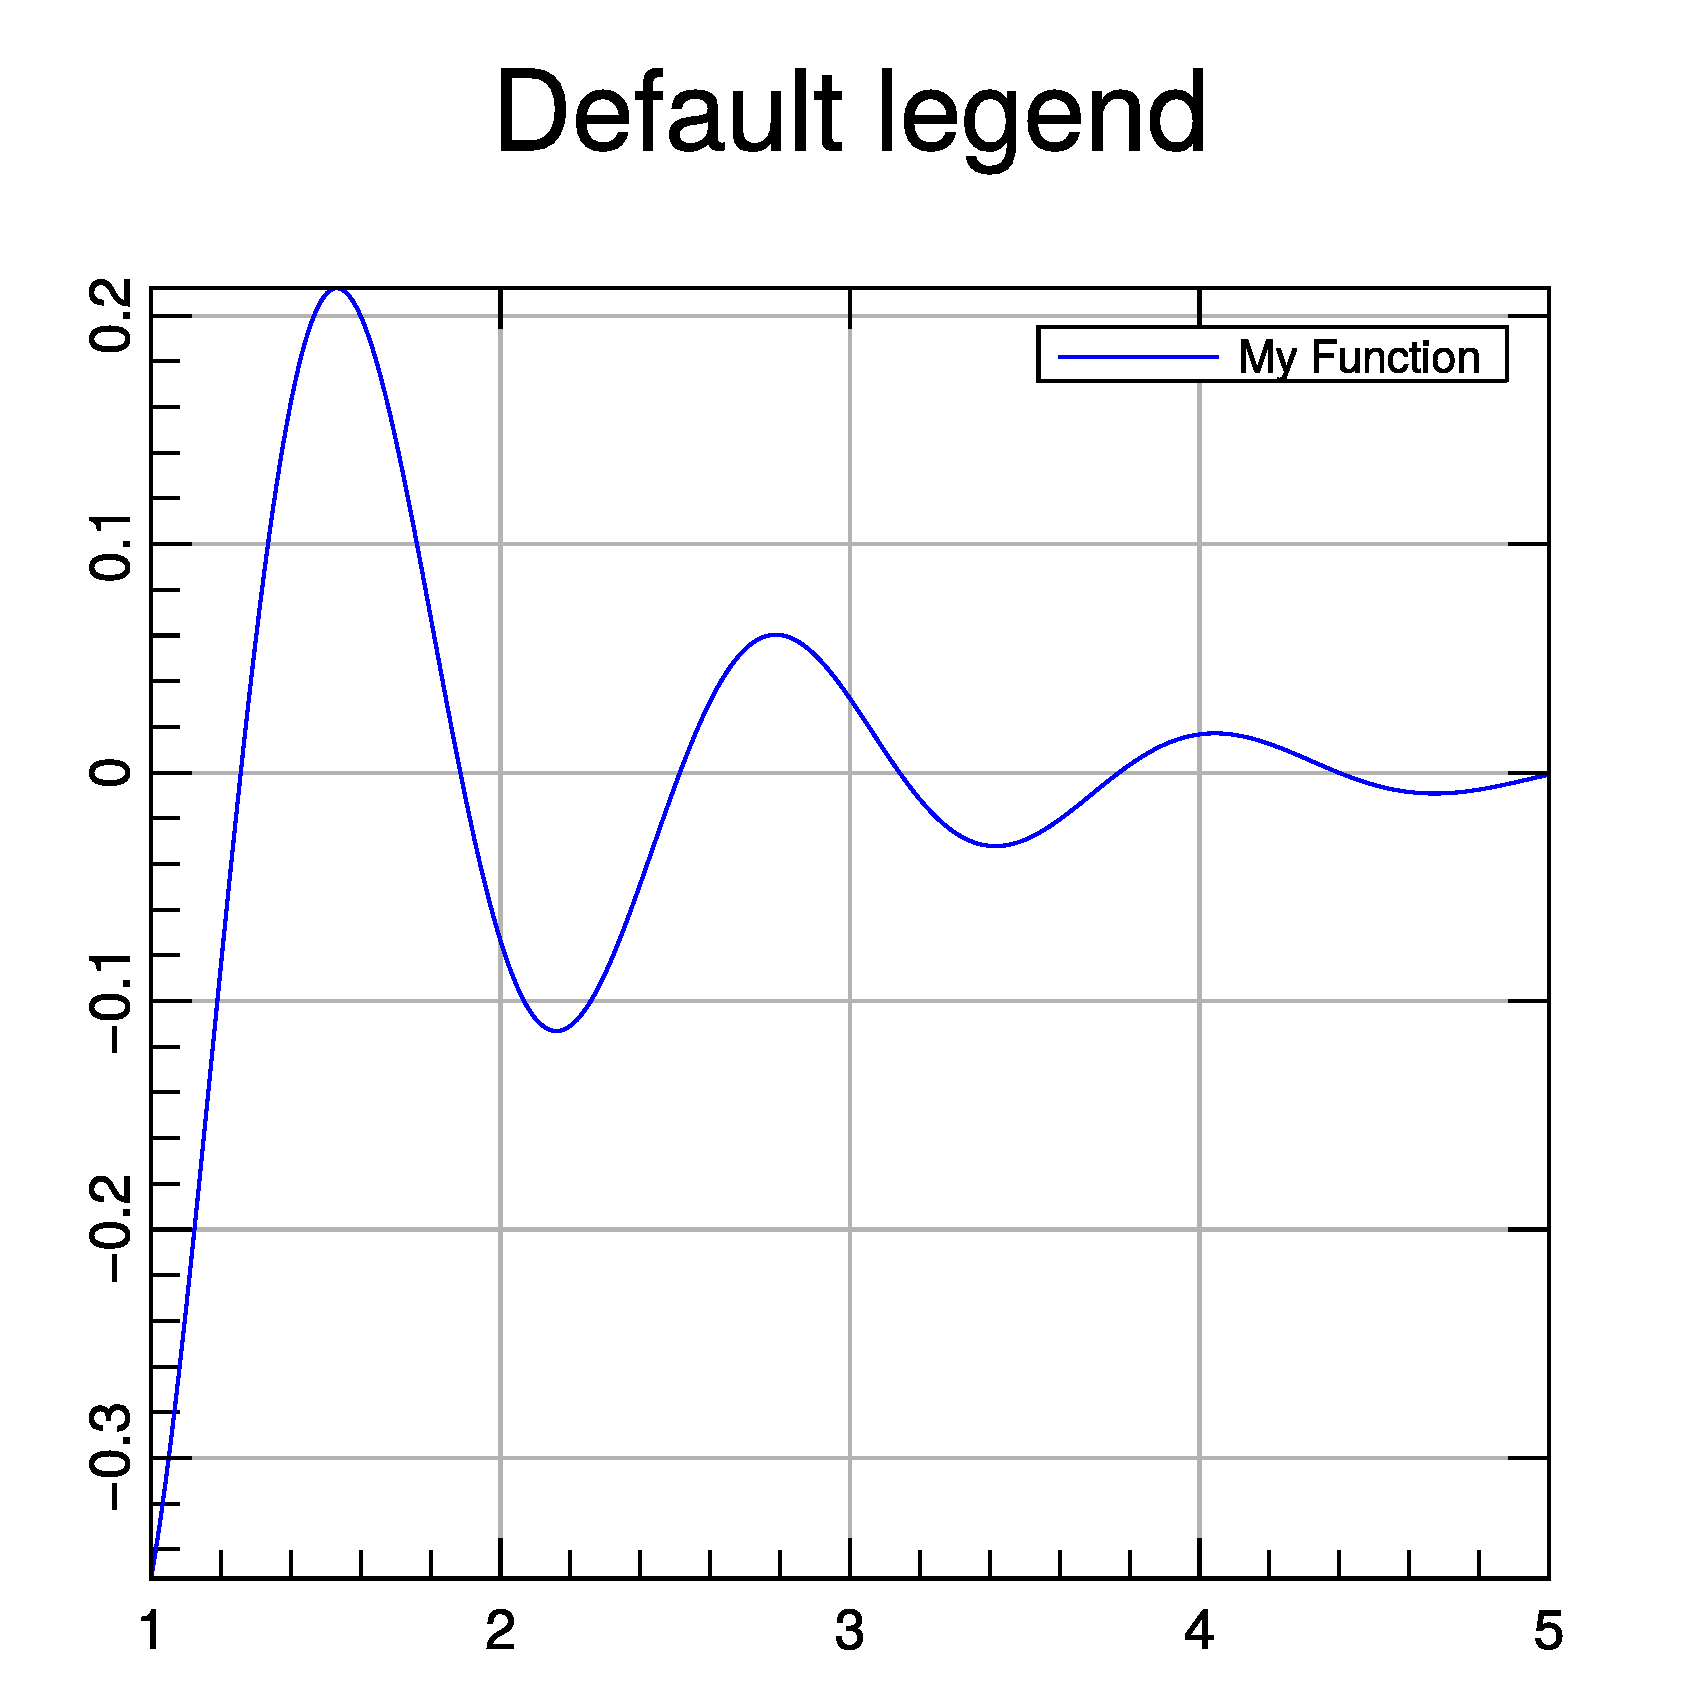
\includegraphics[width=\textwidth]{./examples_from_doc/legend/legend_1.eps}
  \end{subfigure}
  \hspace{2cm}
  \begin{subfigure}[hb]{.32\linewidth}
    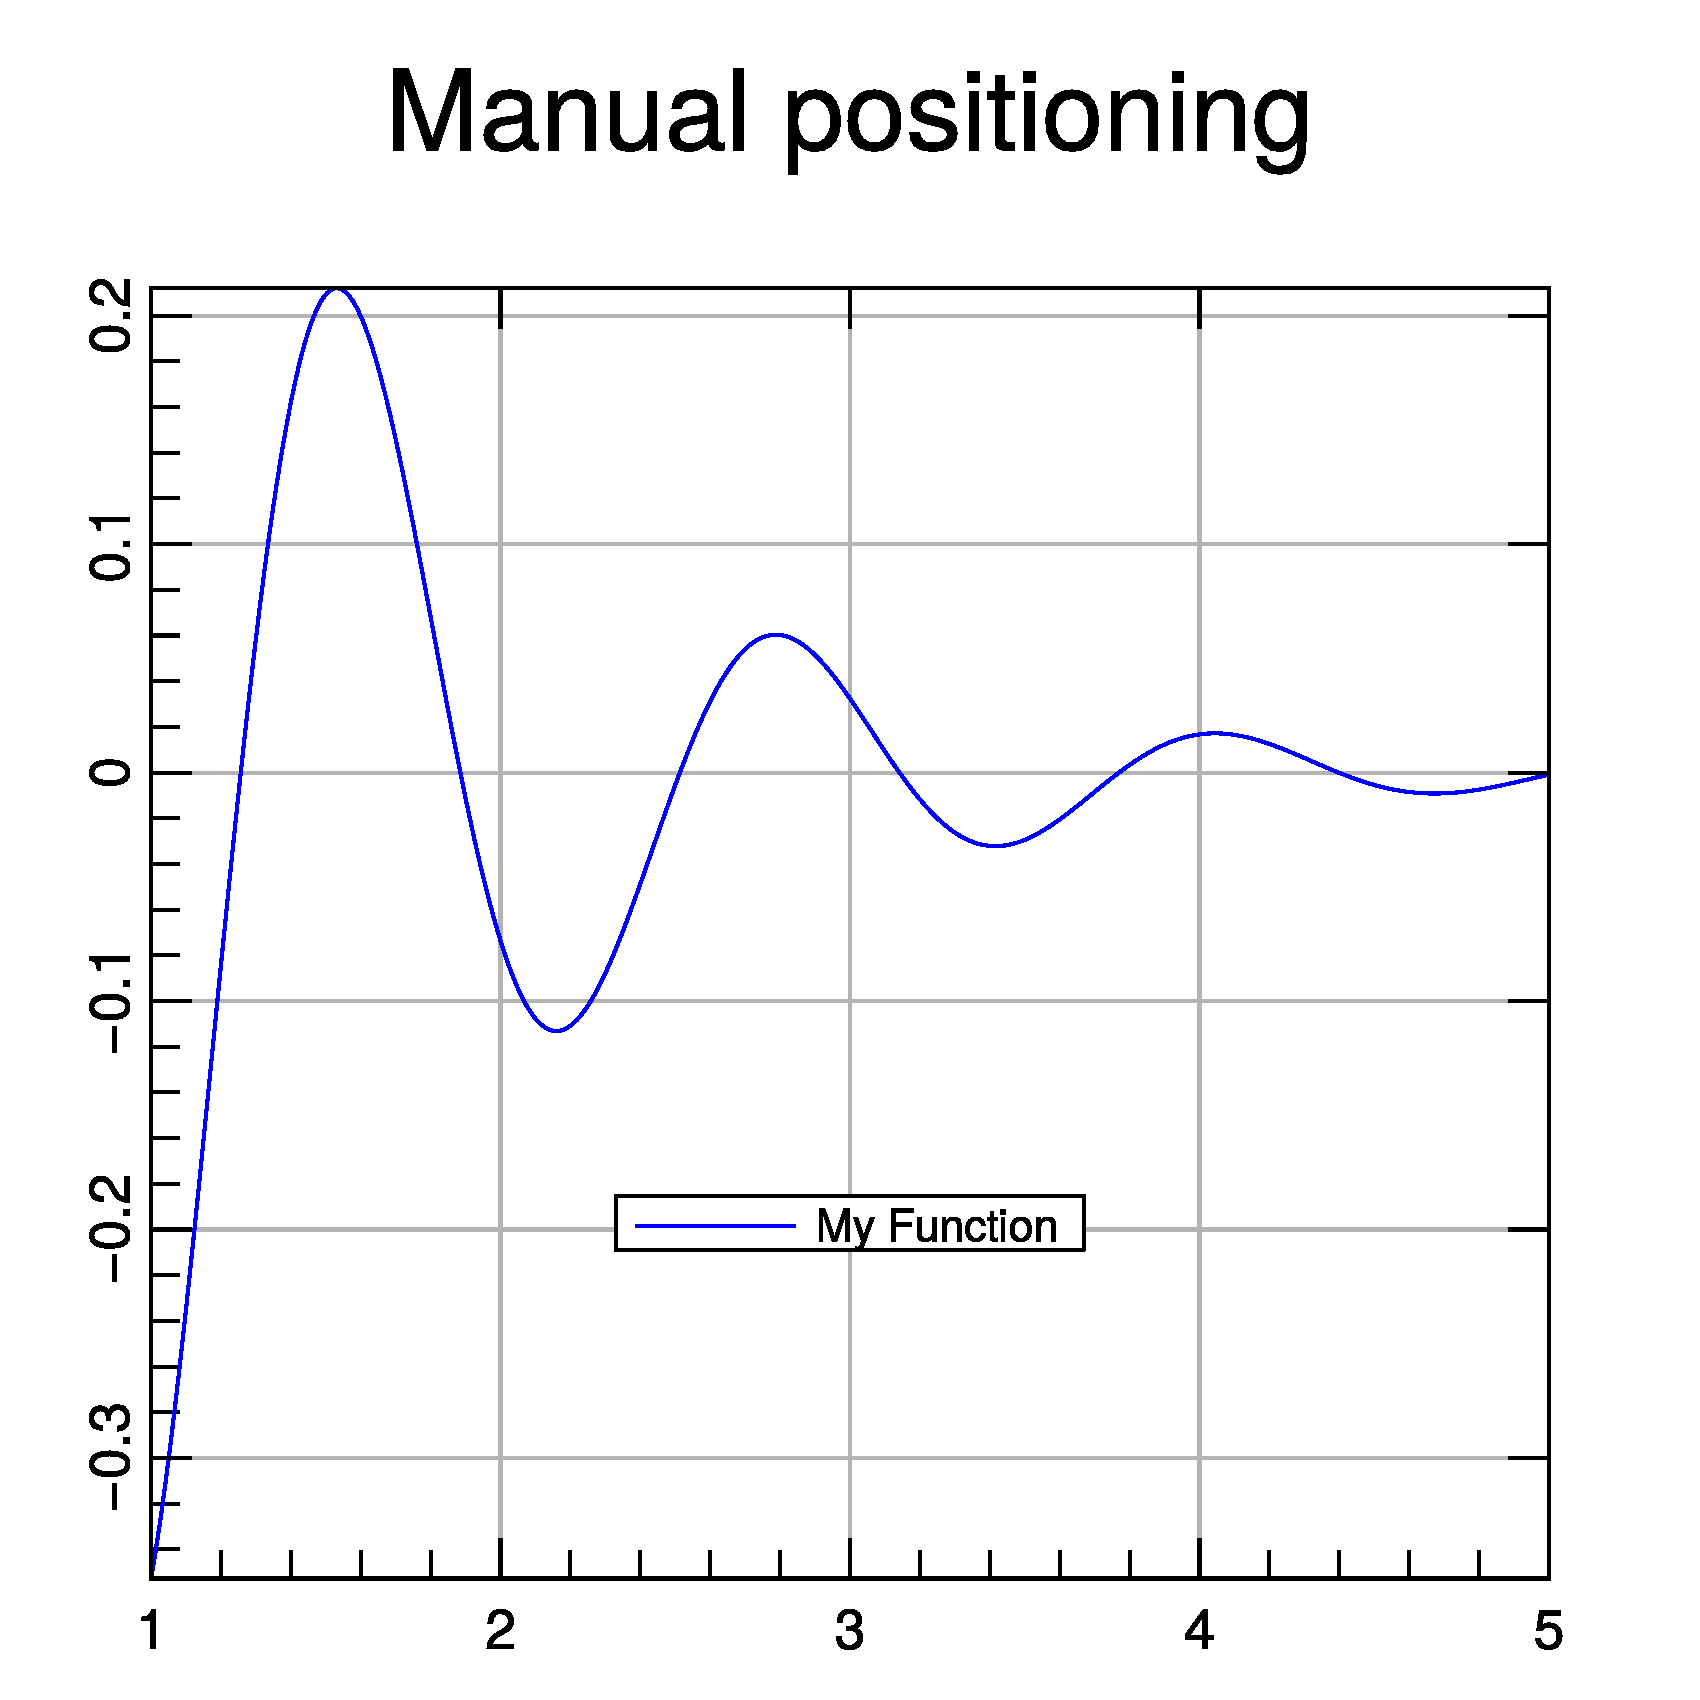
\includegraphics[width=\textwidth]{./examples_from_doc/legend/legend_2.eps}
  \end{subfigure}
\end{figure}

\command{setlog}

\textbf{Definition:}
\begin{lstlisting}
void setlog( const bool& logx = false, 
             const bool& logy = false,
             const bool& logz = false )
\end{lstlisting}
%
\textbf{Restrictions:} All plots will use the latest \texttt{setlog} options or default if none have been set. \\ \\
%
\textbf{Examples:}
\begin{lstlisting}
  mgl::Figure fig;
  fig.[**setlog**](true, false); // -> semilogx
  fig.plot(x0, y0); 
  fig.[**setlog**](false, true); // -> semilogy
  fig.plot(x1, y1);
  fig.[**setlog**](true, true); // -> loglog
  fig.plot(x2, y2);
  fig.save("plot.eps"); // ATTENTION: all plots will have been plotted in loglog-scale 

  mgl::Figure fig;
  fig.plot(x, y);
  fig.save("plot.eps"); // -> default (= linear) scaling
\end{lstlisting}

\begin{figure}[h]
  \centering
  \begin{subfigure}[hb]{.32\linewidth}
    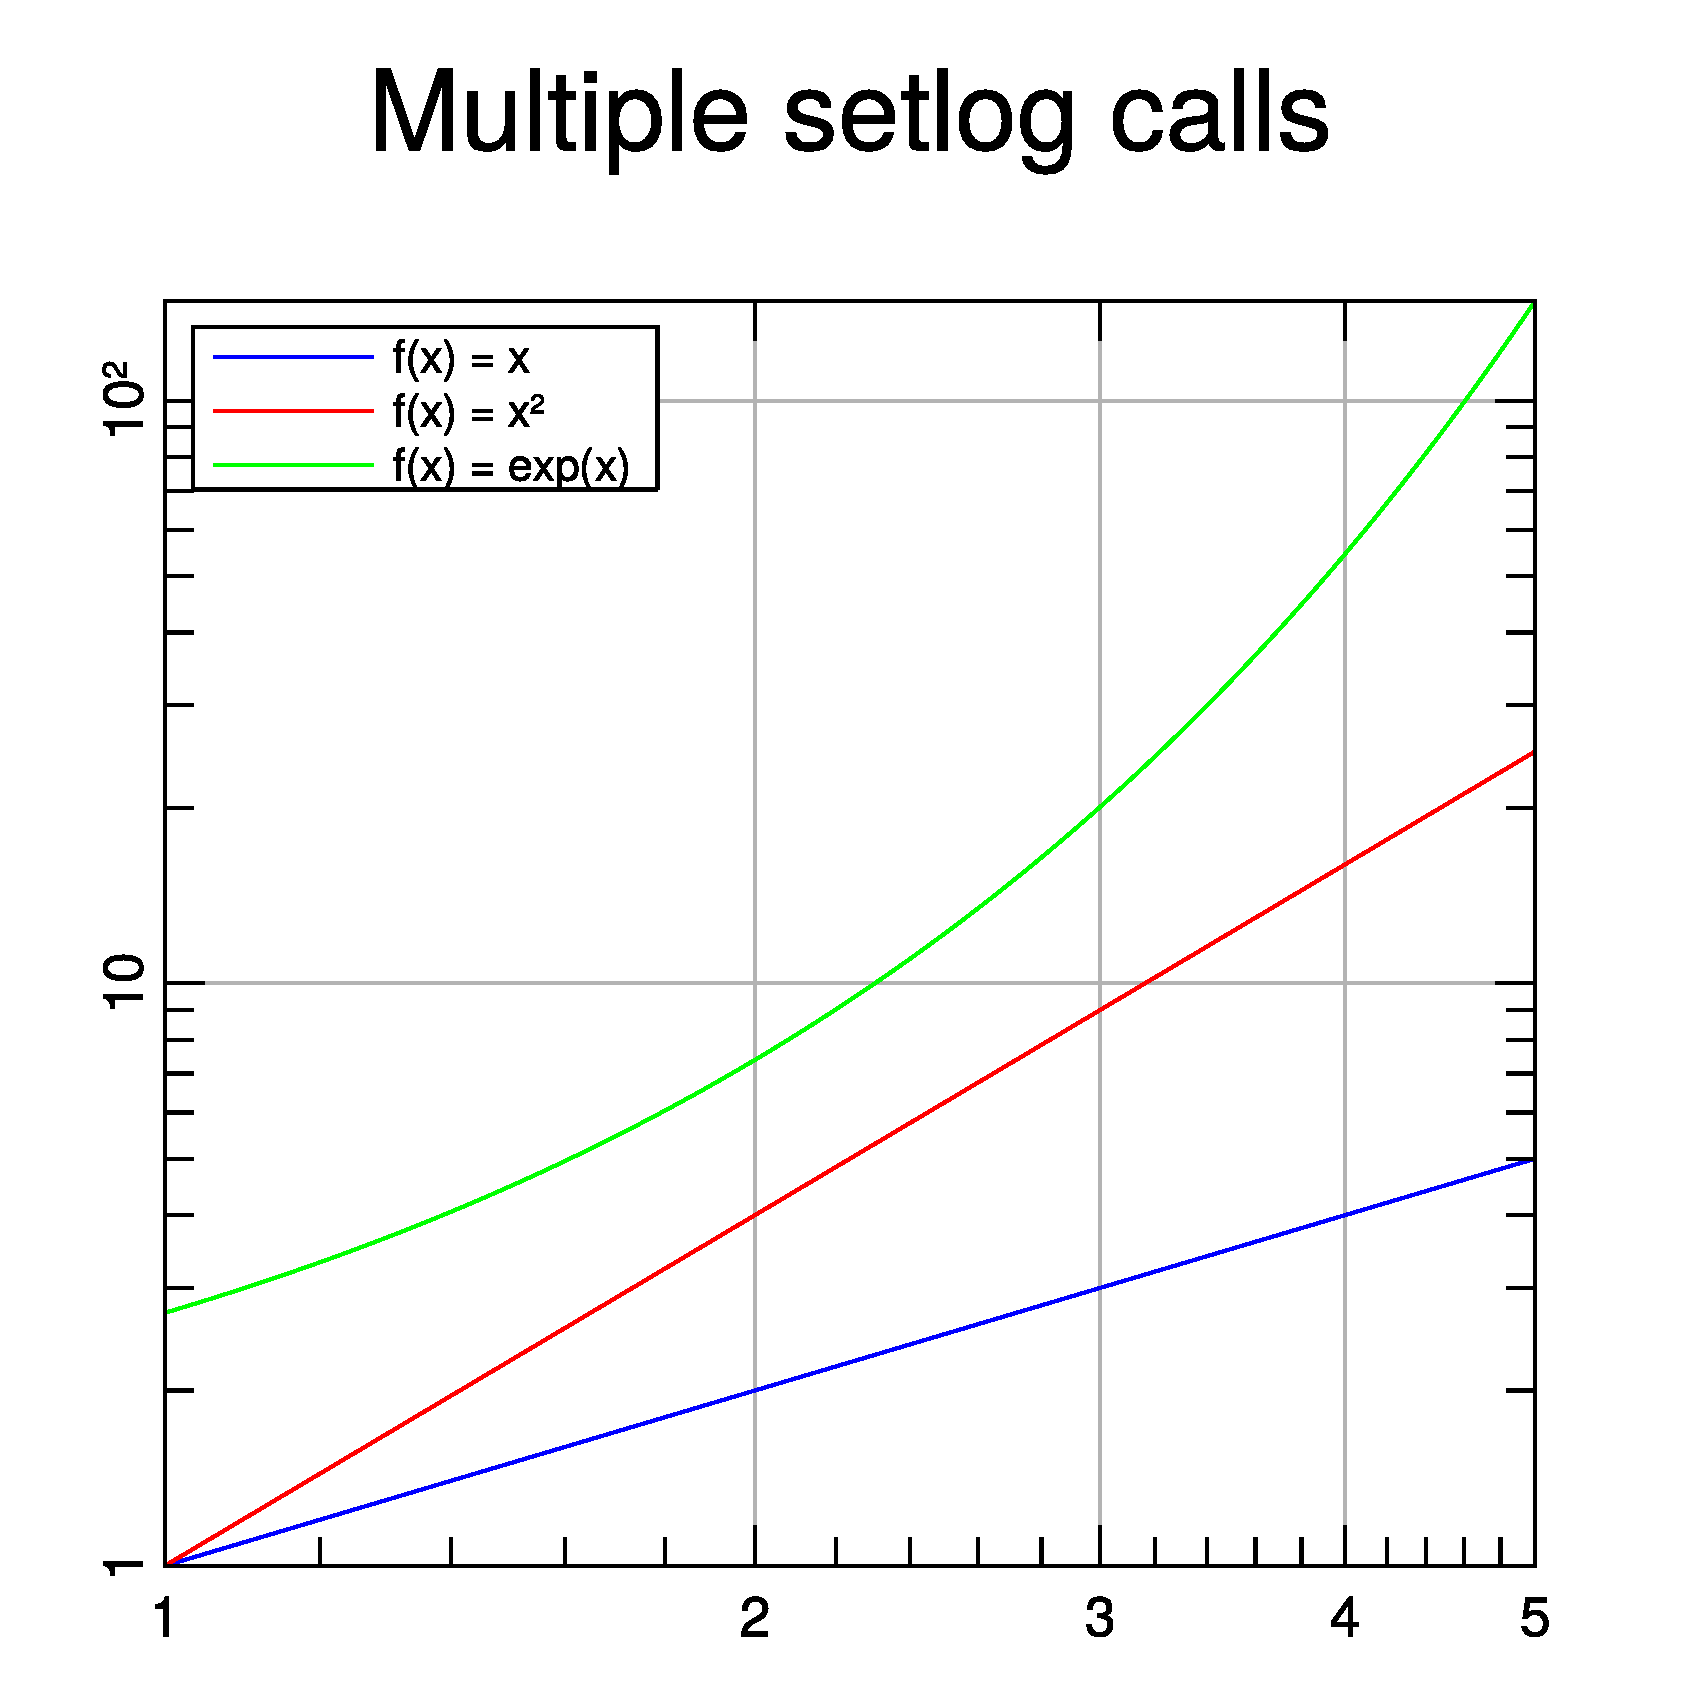
\includegraphics[width=\textwidth]{./examples_from_doc/setlog/setlog_1.eps}
  \end{subfigure}
    \hspace{2cm}
  \begin{subfigure}[hb]{.32\linewidth}
    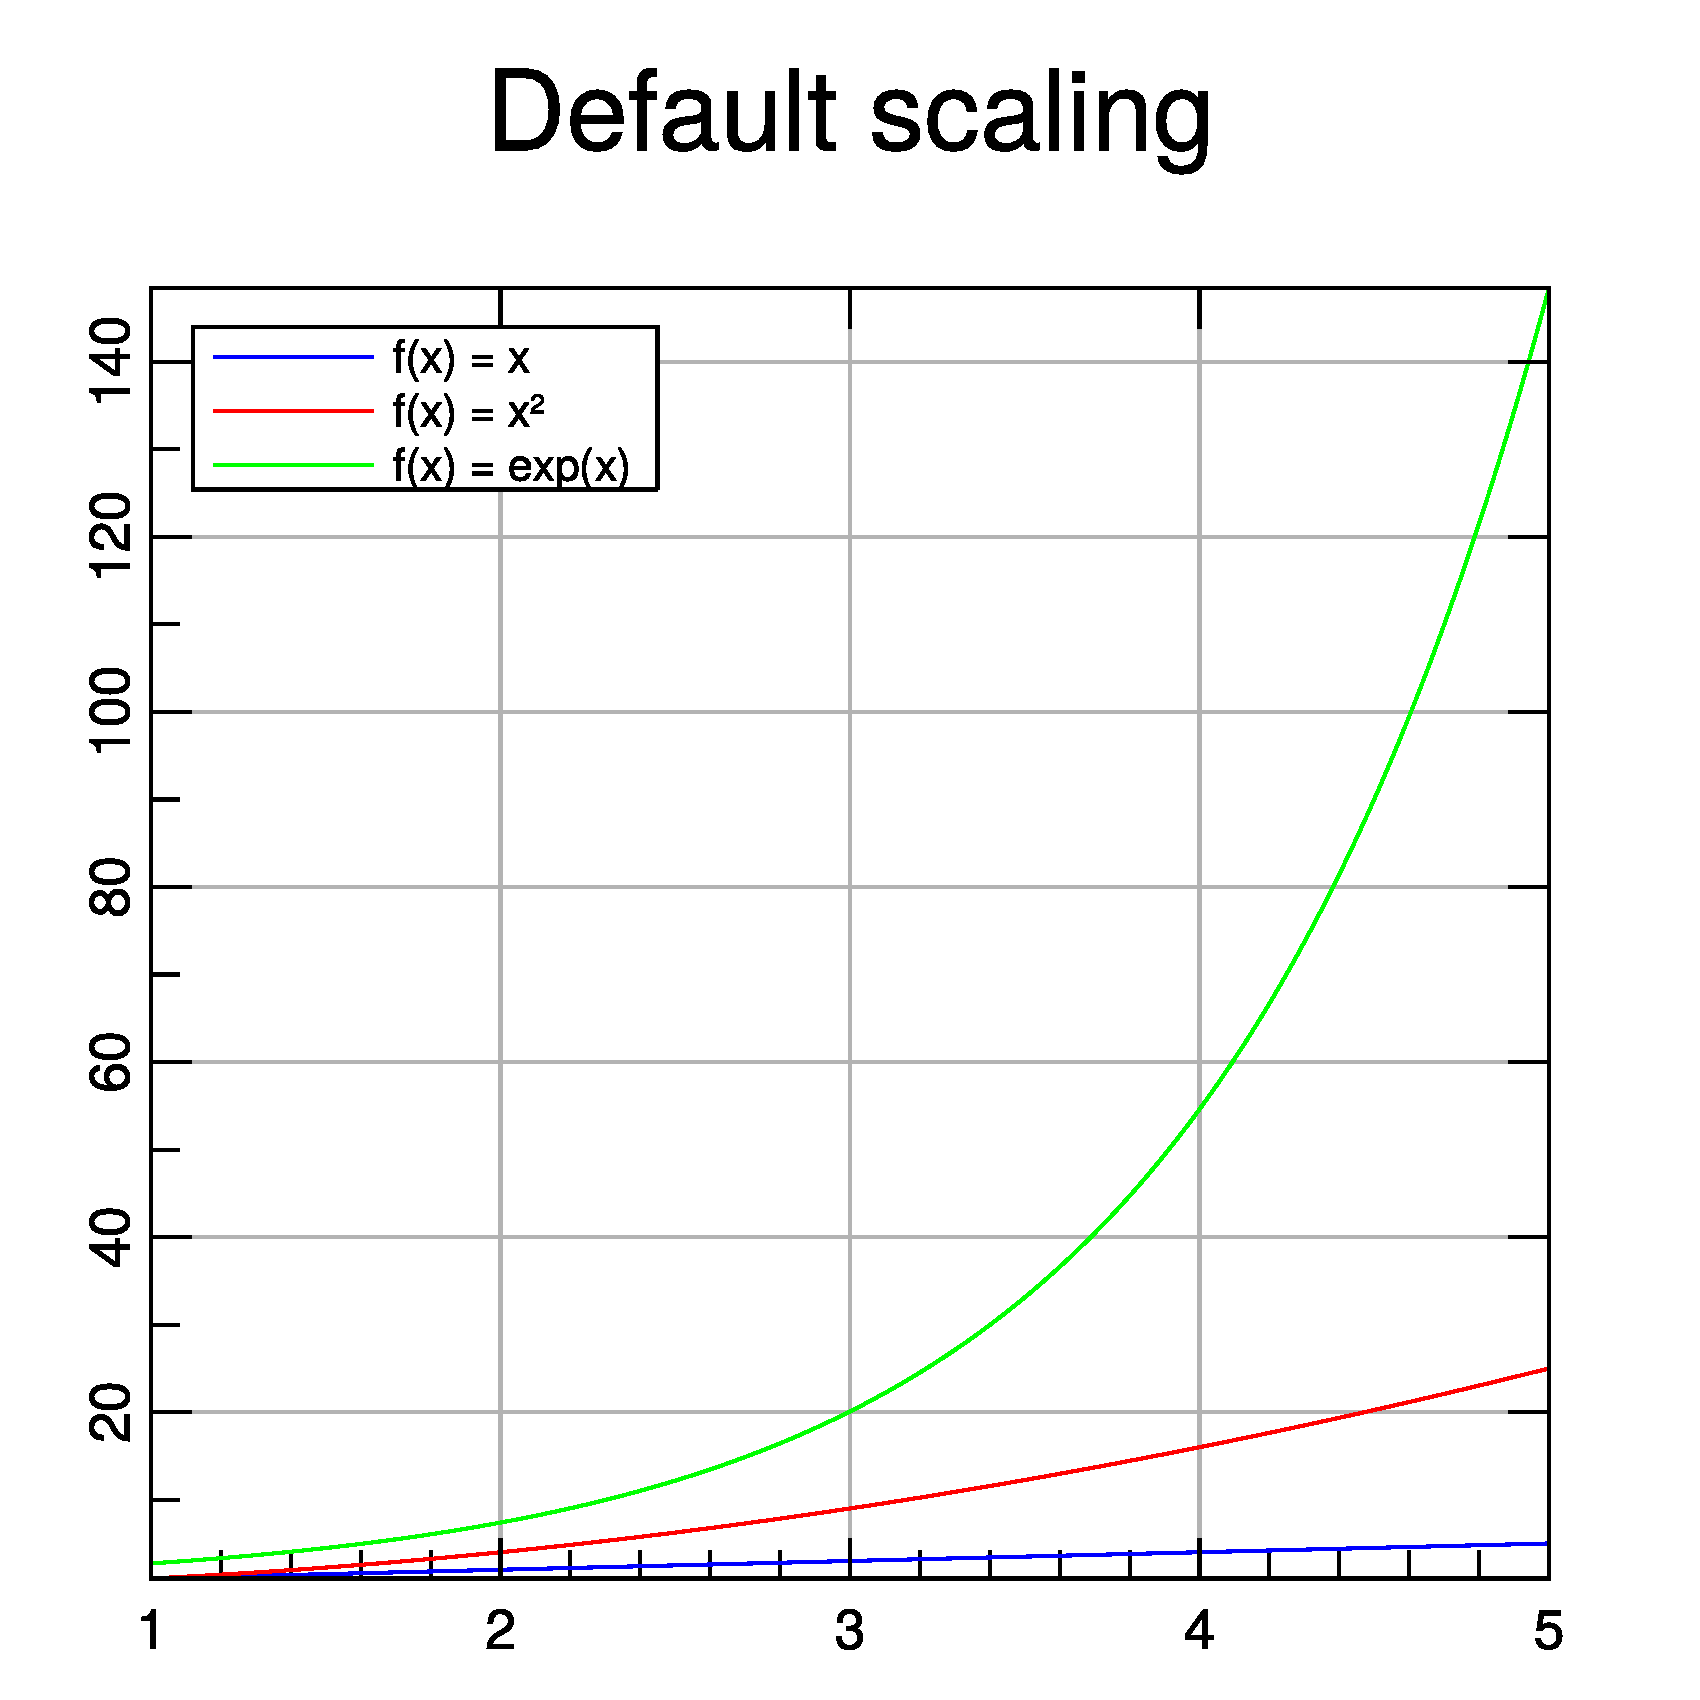
\includegraphics[width=\textwidth]{./examples_from_doc/setlog/setlog_2.eps}
  \end{subfigure}
\end{figure}


\command{plot} 

\textbf{Definition:} 
\begin{lstlisting}
template <typename yVector>
void plot( const yVector& y, 
           const std::string& style = "" )
\end{lstlisting}

\begin{lstlisting}
template <typename xVector, typename yVector>
void plot( const xVector& x, 
           const yVector& y, 
           const std::string& style = "" )
\end{lstlisting}
\textbf{Restrictions:} \texttt{xVector} and \texttt{yVector} must have a \texttt{size()} method, which returns the size of the vector 
and a \texttt{data()} method, which returns a pointer to the first element in the vector. \\
Furthermore \texttt{x} and \texttt{y} must have same length. \\ \\
%
\textbf{Examples:}
\begin{lstlisting}
  mgl::Figure fig;
  fig.[**plot**](x, y, "g;"); // green and dashed linestyle
  fig.save("data.eps");

  mgl::Figure fig;
  fig.[**plot**](x, y); // OK - style is optional
  fig.save("data.eps");

  mgl::Figure fig;
  fig.[**plot**](x, y, " *r", "Data w/ red dots"); // ' *r' equals matlab/python 'r*'
  fig.save("data.eps");
\end{lstlisting}

\begin{figure}[h]
  \centering
  \begin{subfigure}[hb]{.32\linewidth}
    \includegraphics[width=\textwidth]{./examples_from_doc/plot/plot_1.eps}
  \end{subfigure}
    \hfill
  \begin{subfigure}[hb]{.32\linewidth}
    \includegraphics[width=\textwidth]{./examples_from_doc/plot/plot_2.eps}
  \end{subfigure}
    \hfill
  \begin{subfigure}[hb]{.32\linewidth}
    \includegraphics[width=\textwidth]{./examples_from_doc/plot/plot_3.eps}
  \end{subfigure}
\end{figure}


\command{plot3}

\textbf{Definition:}
\begin{lstlisting}
template <typename xVector, typename yVector, typename zVector>
void plot3( const xVector& x,
            const yVector& y,
            const zVector& z,
            const std::string& style = "" )
\end{lstlisting}
\textbf{Restrictions:} Same restrictions as in \texttt{plot} for two vectors, extended to \texttt{zVector}. \\ \\
%
\textbf{Examples:}
\begin{lstlisting}
  mgl::Figure fig;
  fig.[**plot3**](x, y, z);
  fig.save("trajectories.eps");
\end{lstlisting}

\begin{figure}[h]
  \centering
  \begin{subfigure}[hb]{0.45\linewidth}
    \includegraphics[width=\textwidth]{./examples_from_doc/plot3/plot3_1.eps}
  \end{subfigure}
\end{figure}
  

%%%%%%%%%
\newpage
%%%%%%%%%
\command{fplot}

\textbf{Definition:}
\begin{lstlisting}
void fplot( const std::string& function,
            const std::string& style = "" )
\end{lstlisting}
\textbf{Restrictions:} None. \\ \\
%
\textbf{Examples:}
\begin{lstlisting}
  mgl::Figure fig;
  fig.[**fplot**]("(3*x^2 - 4.5/x)*exp(-x/1.3)");
  fig.[**fplot**]("5*sin(5*x)*exp(-x)", "r").label("5sin(5x)*e^{-x}");
  fig.ranges(0.5, 5, -5, 5); // be sure to set ranges for fplot!
  fig.save("plot.eps");

  mgl::Figure fig;
  fig.plot(x, y, "b").label("Benchmark");
  fig.[**fplot**]("x^2", "k;").label("\\ O(x^2)");
  // here we don't set the ranges as it uses the range given by the x,y data
  // and we use fplot to draw a reference line (O(x^2))
  fig.save("runtimes.eps"); 
\end{lstlisting}

\begin{figure}[h]
  \centering
  \begin{subfigure}[hb]{0.32\linewidth}
    \includegraphics[width=\textwidth]{./examples_from_doc/fplot/fplot_1.eps}
  \end{subfigure}
  \hspace{2cm}
  \begin{subfigure}[hb]{0.32\linewidth}
    \includegraphics[width=\textwidth]{./examples_from_doc/fplot/fplot_2.eps}
  \end{subfigure}
\end{figure}

\command{ranges}

\textbf{Definition:}
\begin{lstlisting}
void ranges( const double& xMin, 
             const double& xMax, 
             const double& yMin, 
             const double& yMax )
\end{lstlisting}
%
\textbf{Restrictions:} xMin $<$ xMax, yMin $<$ yMax and ranges must be $>$ 0 for axis in logarithmic scale. \\ \\
%
\textbf{Examples:}
\begin{lstlisting}
  mgl::Figure fig;
  fig.[**ranges**](-1,1,-1,1);
  fig.plot(x, y, "b");

  mgl::Figure fig;
  fig.plot(x, y, "b");
  fig.[**ranges**](0, 2.3, 4, 5); // ranges can be called before or after 'plot'

  mgl::Figure fig;
  fig.[**ranges**](-1, 1, 0, 5);
  fig.setlog(true, true); // will run but MathGL will throw a warning 
  fig.plot(x, y, "b");
\end{lstlisting}

\begin{figure}
  \centering
  \begin{subfigure}[hb]{0.32\linewidth}
    \includegraphics[width=\textwidth]{./examples_from_doc/ranges/ranges_1.eps}
  \end{subfigure}
  \hfill
  \begin{subfigure}[hb]{0.32\linewidth}
    \includegraphics[width=\textwidth]{./examples_from_doc/ranges/ranges_2.eps}
  \end{subfigure}
  \hfill
  \begin{subfigure}[hb]{0.32\linewidth}
    \includegraphics[width=\textwidth]{./examples_from_doc/ranges/ranges_3.eps}
  \end{subfigure}
\end{figure}

\command{save}

\textbf{Definition:}
\begin{lstlisting}
void save( const std::string& file )
\end{lstlisting}
%
\textbf{Restrictions:} Supported file formats: \texttt{.eps} and \texttt{.png}. \\ \\
%
\textbf{Examples:}
\begin{lstlisting}
  mgl::Figure fig;
  fig.[**save**]("plot.eps"); // OK

  mgl::Figure fig;
  fig.[**save**]("plot"); // OK - will be saved as plot.eps

  mgl::Figure fig;
  fig.[**save**]("plot.png"); // OK - but needs -lpng flag!
\end{lstlisting}

\command{title}

\textbf{Definition:}
\begin{lstlisting}
void title( const std::string& text )
\end{lstlisting}
%
\textbf{Restrictions:} None.

\section{Line characteristics}

\begin{minipage}{3cm}
  Linecolors\footnote{
  Upper-case letters will give a darker version of the lower-case version.
  }:\\ \\
  \begin{tabular}{l|c}
    \textcolor{blue}{blue} & \texttt{b} \\
    \textcolor{green}{green} & \texttt{g} \\
    \textcolor{red}{red} & \texttt{r} \\
    \textcolor{cyan}{cyan} & \texttt{c} \\
    \textcolor{magenta}{magenta} & \texttt{m} \\
    \textcolor{yellow}{yellow} & \texttt{y} \\
    \textcolor[gray]{0.5}{gray} & \texttt{h} \\
    \textcolor{SeaGreen}{green-blue} & \texttt{l} \\
    \textcolor{RoyalBlue}{sky-blue} & \texttt{n} \\
    \textcolor{orange}{orange} & \texttt{q} \\
    \textcolor{LimeGreen}{green-yellow} & \texttt{e} \\
    \textcolor{CadetBlue}{blue-violet} & \texttt{u} \\
    \textcolor{purple}{purple} & \texttt{p}
  \end{tabular}
\end{minipage}
\hfill
\begin{minipage}{4cm}
  Linestyles:\\ \\
  \begin{tabular}{l|c}
    none & \\
    solid & \texttt{-} \\
    dashed & \texttt{;} \\
    small dashed & \texttt{=} \\
    long dashed & \texttt{|} \\
    dotted & \texttt{:} \\
    dash-dotted & \texttt{j} \\
    small dash-dotted & \texttt{i} 
  \end{tabular}
  None is used as follows: \\
  \texttt{" r*"} gives red stars w/o any lines
\end{minipage}
\hfill
\begin{minipage}{2cm}
  Linemarkers:\\ \\
  \begin{tabular}{l|c}
    + & \texttt{+} \\
    o & \texttt{o} \\
    $\diamond$ & \texttt{d} \\
    $\cdot$ & \texttt{.} \\
    $\triangle$ & \texttt{\^{}} \\
    $\nabla$ &\texttt{v} \\
    $\lhd$ & \texttt{<} \\
    $\rhd$ & \texttt{>} \\
    $\odot$ & \texttt{\#.} \\
    $\boxplus$ & \texttt{\#+} \\
    $\boxtimes$ & \texttt{\#x} 
  \end{tabular}
\end{minipage}



\end{document}
